\documentclass{beamer}
\usepackage[utf8]{inputenc}
\usetheme{Copenhagen}
\usepackage[spanish]{babel}
\usepackage{multirow}
%\usepackage{estilo-apuntes}
\usepackage{braids}
\usepackage[]{graphicx}
\usepackage{rotating}
\usepackage{pgf,tikz}
\usepackage{pgfplots}
\usepackage{tikz-cd}
\usetikzlibrary{arrows}
\usetikzlibrary{cd}
\usetikzlibrary{babel}
\pgfplotsset{compat=1.13}
\usetikzlibrary{decorations.shapes}
\pgfkeyssetvalue{/tikz/braid height}{1cm} %no parece hacer nada
\pgfkeyssetvalue{/tikz/braid width}{1cm}
\pgfkeyssetvalue{/tikz/braid start}{(0,0)}
\pgfkeyssetvalue{/tikz/braid colour}{black}

\theoremstyle{definition}

\newtheorem{teorema}{Teorema}
\newtheorem{defi}{Definición}
\newtheorem{prop}[teorema]{Proposición}

\newcommand{\Z}{\mathbb{Z}}
\newcommand{\C}{\mathbb{C}}
\newcommand{\D}{\mathbb{D}}
\providecommand{\gene}[1]{\langle{#1}\rangle}


\addtobeamertemplate{navigation symbols}{}{%
    \usebeamerfont{footline}%
    \usebeamercolor[fg]{footline}%
    \hspace{1em}%
    \insertframenumber/\inserttotalframenumber
}
\setbeamercolor{footline}{fg=black}
\setbeamerfont{footline}{series=\bfseries}

%-----------------------------------------------------------

\title{Funcionamiento de Bitcoin}
\author{Javier Aguilar Martín y Jesús López Sánchez}
\institute{Universidad de Sevilla}
\date{}
 
\begin{document}
\frame{\titlepage}
%\begin{frame}
%
%
%\title[About Beamer] %optional
%{About the Beamer class in presentation making}
% 
%\subtitle{A short story}
% 
%\author[Arthur, Doe] % (optional, for multiple authors)
%{A.~B.~Arthur\inst{1} \and J.~Doe\inst{2}}
% 
%\institute[VFU] % (optional)
%{
%  \inst{1}%
%  Faculty of Physics\\
%  Very Famous University
%  \and
%  \inst{2}%
%  Faculty of Chemistry\\
%  Very Famous University
%}

% 
%\date[VLC 2013] % (optional)
%{Very Large Conference, April 2013}


%\end{frame}
\setbeamercovered{highly dynamic}

\newcounter{saveenumi}
\newcommand{\seti}{\setcounter{saveenumi}{\value{enumi}}}
\newcommand{\conti}{\setcounter{enumi}{\value{saveenumi}}}

\resetcounteronoverlays{saveenumi}
%\AtBeginSection[]{
\begin{frame}
\frametitle{Tabla de contenidos}
\tableofcontents
\end{frame}
%}

%\begin{frame}
%	%AÑADIR ESTAS URL AL FINAL POR SI ME DA TIEMPO ENSEÑAR ESTAS COSAS 
%	%\url{https://www.blockchain.com/btc/blocks}
%	%\url{https://coin.dance/blocks}
%	%\url{https://www.blockchain.com/btc/unconfirmed-transactions}
%	
%%	ESTE TENGO PRIMERO QUE MIRARLO PARA HACERLO YO
%%	\url{https://anders.com/blockchain/}
%
%\end{frame}

\section{Overview}
\begin{frame}
	\frametitle{Overview}
	\begin{itemize}
		\item<1-> Bitcoin es una criptomoneda sin banco central creada en 2008 por el seudónimo Satoshi Nakamoto. La red P2P controla los procesos de forma distribuida.
		\item<2-> Cada usuario de Bitcoin tiene una dirección (clave pública) con la que recibe Bitcoins y una clave privada con la que los gasta.
		\item<3-> Cada intercambio de Bitcoins se llama transacción.
		\item<4-> Las transacciones se almacenan en una cadena de bloques (blockchain) creada por ``mineros'' que sirve como libro de cuentas.
		\item<5-> Bitcoin usa el algoritmo de firma digital sobre la curva elíptica secp256k1, que tiene ecuación $y^2 = x^3 + 7$ y está definida sobre el cuerpo $\mathbb{F}_p$ con $p$ del orden de $2^{256}$.
	\end{itemize}
	
	
	
	
	
	
	
\end{frame}



\section{Preliminares}
\subsection{Firma digital sobre curvas elípticas}
\begin{frame}
\frametitle{Generación de claves}
\begin{itemize}
	\item<1-> Se fija un punto base $P$ de orden $N$ (primo grande).
	\item<2-> Se elige como clave privada un número aleatorio $x\in\{2,\dots, N-1\}$.
	\item<3-> Calculamos la clave pública $Y=xP$.
\end{itemize}


\only<4>{\begin{alertblock}{}
	$N$ marca el número máximo de claves públicas y por tanto de direcciones de Bitcoin.
\end{alertblock}}
\end{frame} 

\begin{frame}
	\frametitle{Firma digital sobre curvas elípticas}
	Para firmar un mensaje $m$ usando el algoritmo sobre curvas elípticas se hace lo siguiente:
\begin{itemize}
	\item<2-> Dada una función hash $h$, calcular $e=h(m)$.
	\item<3-> Tomar $z$ el conjunto de $l$ dígitos más a la izquierda de $e$, donde $l$ es la longitud en bits de $N$.
	\item<4-> Elegir un número entero aleatorio $k\in\{1,\dots,N-1\}$.
	\item<5-> Calcular el punto $(a,b)=kP$.
	\item<6-> Calcular $r\equiv a\mod N$. Si $r=0$, vuelta al paso 3.
	\item<7-> Calcular $s\equiv (z+rx)k^{-1}\mod N$. Si $s=0$, vuelta al paso 3. 
	\item<8-> La firma es el par $(r,s)$.
\end{itemize}
\end{frame}

\begin{frame}
\frametitle{Verificación de la firma}
En primer lugar se verifica que la clave pública $Y$ es válida:
\begin{itemize}
	\item<2-> Comprobar que $Y$ no es el punto base.
	\item<3-> Comprobar que $Y$ es un punto de la curva.
	\item<4-> Comprobar que el orden de $Y$ es $N$.
\end{itemize} 
\end{frame}

\begin{frame}
A continuación, se verifica la firma:
\begin{itemize}
	\item<1-> Verificar que $1\leq r,s\leq N-1$.
	\item<2-> Calcular $e=h(m)$.
	\item<3-> Tomar $z$ como los $l$ bits más a la izquierda de $e$.
	\item<4-> Calcular $w\equiv s^{-1}\mod N$.
	\item<5-> Calcular $u\equiv zw\mod N$ y $v\equiv rw\mod N$. 
	\item<6-> Calcular el punto $(a,b)=uP+vY$. Si el punto es el origen, la firma es inválida.
	\item<7-> Verificar que $r\equiv a\mod N$. La firma es inválida en caso contrario.
\end{itemize}	
\end{frame}



\subsection{Árboles de Merkle}

\begin{frame}
	\frametitle{Árboles de Merkle}
	\begin{defi}
		Los \textbf{árboles de Merkle} son árboles binarios de hashes usados para verificar eficientemente la integridad de los datos.
	\end{defi}
\begin{figure}[h!]
	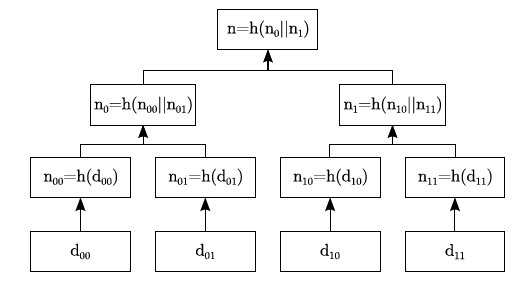
\includegraphics[scale=0.5]{merkle}
\end{figure}
%Lo de abajo del todo son datos, las hojas están justo encima
\end{frame}
\begin{frame}
	\begin{itemize}
		\item<1-> Las hojas se calculan directamente como hash de los bloques de datos, mientras que el resto de los nodos se calculan como hash de la concatenación de sus hijos.
		\item<2-> Cuando cambia un bloque de datos no es necesario calcular el hash sobre todos los datos, solo hace falta recalcular desde la modificación hasta la raíz. 
		\item<3-> Si hay un número impar de nodos en una fila, el último se duplica.
	\end{itemize}
\end{frame}

\subsection{Prueba de Trabajo}
\begin{frame}
\frametitle{Prueba de trabajo}
\begin{defi}
	Una \textbf{prueba de trabajo} es un reto criptográfico para asegurar que una parte ha realizado una determinada cantidad de trabajo computacional. La verificación de la prueba debe poder realizarse de forma eficiente.
\end{defi}\pause

Supongamos que Alice quiere pedirle a Bob que realice un trabajo computacional en cada mensaje que le envíe. Alice puede pedirle a Bob una cadena de texto cuyo hash verifique una cierta estructura. Encontrar esa cadena tiene una probabilidad de acierto que determinará la cantidad media de trabajo realizada por Bob.
\end{frame}

\begin{frame}
	\frametitle{Prueba de trabajo de Bitcoin}
	\begin{itemize}
	\item<1-> Bitcoin utiliza como algoritmo de hash el doble $SHA256$ ($SHA256^2$).
	\item<2-> La estructura predefinida es que el hash (en hexadecimal) sea menor o igual que un valor $T$.
	\item<3-> Para un mensaje $m$, la probabilidad de encontrar un \textbf{nonce} $n$ que verifique $H=SHA256^2(m||n)\leq T$ es
	$$P(H\leq T)=\frac{T}{2^{256}}$$
	\item<4-> La verificación de la prueba consiste simplemente en comprobar $SHA256^2(m||n)\leq T$.
	\end{itemize}
\end{frame}

\begin{frame}
\frametitle{Importancia de la prueba de trabajo en Bitcoin}
\begin{itemize}
	\item Permite que el Bitcoin se distribuya aleatoriamente en función del poder computacional. %por ser aleatorio
	\item Protege a la red frente ataques maliciosos. %porque hace falta trabajo
\end{itemize}
\end{frame}


\section{Transacciones}
\subsection{Transacciones regulares}
\begin{frame}
\frametitle{Transacciones regulares}
\begin{defi}
	Una \textbf{transacción regular} es una transferencia de Bitcoins entre usuarios distintos. Coniste en un archivo que contiene los siguientes datos: un número de versión ($nVersion$), un vector de inputs ($vin$), un vector de outputs ($vout$) y una fecha ($nLockTime$). Incluye además $\# vin$ y $\# vout$ (el número de elementos de $vin$ y $vout$, respectivamente), y una comisión ($fee$). 
\end{defi}

\end{frame}

\begin{frame}
	\begin{figure}
		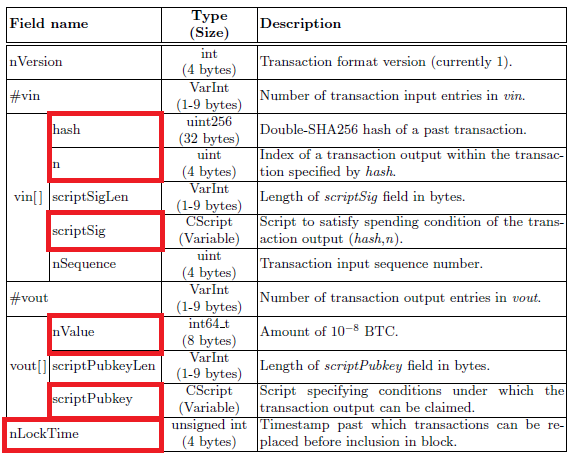
\includegraphics[scale=0.5]{regular}
	\end{figure}
\end{frame}


\begin{frame}
%	\begin{block}{nVersion}
%		Almacena el número de versión del formato de transacción. Actualmente es 1.
%	\end{block}\pause

\begin{block}{vin}
	Almacena un vector con una o más transacciones. Cada input está compuesto por una referencia a un output previo ($hash,n$), el campo de firma ($scriptSig$), la longitud del campo de firma en bytes ($scriptSigLen$) y un número de secuencia de transacción ($nSequence$).
\end{block}
\end{frame}

\begin{frame}
\begin{itemize}
	\item<1-> $(hash,n)$: un output previo se identifica con la tupla $(hash,n)$. El campo $hash$, o \textbf{ID de transacción} ($TxID$) se calcula como el doble $SHA256$ de la transacción anterior: $$TxID=SHA256^2(Transaction)$$
	El valor $n$ almacenado en el $vout$ de la transacción anterior es la cantidad de Bitcoin transferida.
	
		\item<2-> $scriptSig$: contiene la firma digital de los inputs de la transacción (es decir, los outputs de la transacción anterior).
		
	
\end{itemize}
\end{frame}

\begin{frame}
	\begin{figure}
		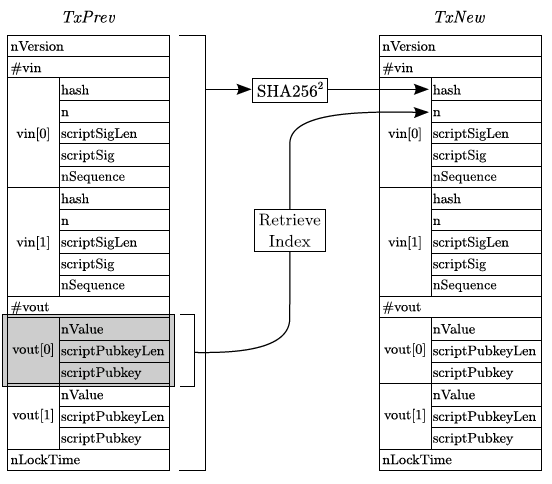
\includegraphics[scale=0.5]{hash}
	\end{figure}
\end{frame}


\begin{frame}
	\begin{block}{vout}
		Almacena un vector con una o más transacciones output. Cada transacción output está compuesta por una cantidad de BTC para ser gastada ($nValue$), la clave pública ($scriptPubkey$) y la longitud de la clave pública ($scriptPubkeyLen$).
	\end{block}
\begin{itemize}
	\item<2-> $nValue$: almacena la cantidad de BTC transferida. Esta cantidad está representada en \textbf{Satoshis}, esto es $10^{-18}$ BTC.
	\item<3->$scriptPubkey$: es un espacio en el que se introduce la clave pública del destinatario, quien debe probar mediante una prueba de conocimiento que su clave privada se corresponde a dicha clave pública.
\end{itemize}
	
\end{frame}

\begin{frame}

	\begin{block}{nLockTime}
		Almacena un tiempo de bloqueo, es decir, el momento (en formato UNIX) a partir del cual la transacción debería ser incluida en un bloque.
	\end{block}\pause

\begin{block}{fee}
	Las transacciones incluyen también una comisión máxima que sirve de incentivo para que los mineros las incluyan la transacción en sus bloques. La transacción efectiva depende de la diferencia entre la suma de los inputs y los outputs.
\end{block}

\end{frame}
\begin{frame}
	\href{https://api.blockcypher.com/v1/btc/main/txs/0142f951d09eb4df18eeff1879d548974f3afd6b94443dff5b2aba4ce5d5a403?limit=50&includeHex=true}{Ejemplo de transacción real} 
	
\end{frame}
\subsection{Transacciones Coinbase}
\begin{frame}
	\frametitle{Transacciones Coinbase}
	\begin{defi}
		Las \textbf{transacciones Coinbase} son las transacciones mediante las que los Bitcoin se introducen en el sistema. Estas transacciones van siempre en primer lugar en los bloques. 
	\end{defi}\pause

Tienen la misma estructura que las transacciones regulares pero con ligeras modificaciones y algunas restricciones.
\end{frame}

\begin{frame}

	\begin{figure}
		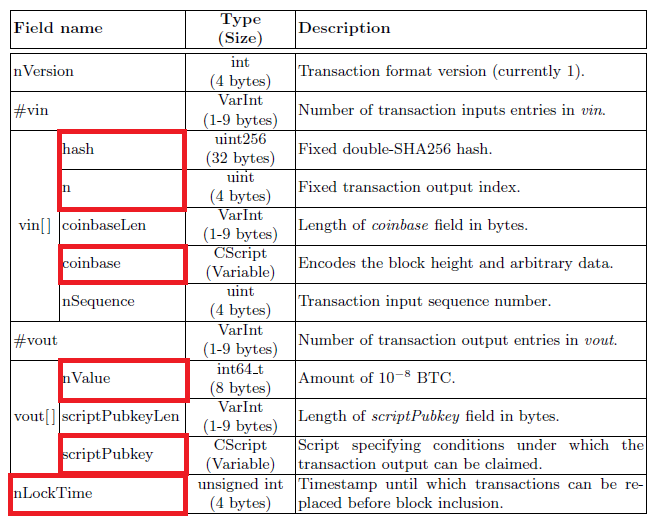
\includegraphics[scale=0.5]{coinbase}
	\end{figure}
\end{frame}

\begin{frame}
	\begin{block}{vin}
		Almacena una sola transacción. El input está formado por una referencia $(hash, n)$ a una transacción output concreta, el campo $coinbase$ junto con su longitud ($coinbaseLen$) y un número de secuencia de transacción ($nSequence$).
	\end{block}
\end{frame}

\begin{frame}
	\begin{itemize}
		\item<1-> $(hash,n)$: como las transacciones coinbase introducen Bitcoin en el sistema, no hay transacciones previas a la que referirse, por lo que este campo almacena los valores constantes $hash=0$, $n=2^{32}-1$. 
		\item<2-> $coinbase$: almacena la altura del bloque, es decir, la posición del bloque en la blockchain, y datos arbitrarios. 
	\end{itemize}

\end{frame}

\begin{frame}
	\begin{block}{vout}
		El vector de output está restringido por la cantidad máxima de Bitcoin que se puede transferir.
	\end{block}\pause

\begin{itemize}
	\item $nValue$: en una transacción coinbase el minero está autorizado a reclamar un subsidio de minería, así como las comisiones de todas las transacciones incluidas, como recompensa por resolver la prueba de trabajo. El subsidio de minería es actualmente de 12.5BTC, y se divide por la mitad cada 210000 bloques. 
\end{itemize}

\end{frame}

\section{Blockchain}
\subsection{Bloques}
\begin{frame}
	\frametitle{Bloques}
	\begin{defi}
		Un \textbf{bloque} es un archivo que contiene una colección de transferencias. Los bloques están formados por un \textbf{encabezado} (header) y una \textbf{carga útil} (payload). El encabezado almacena su versión ($nVersion$), una referencia al bloque anterior ($HashPrevBlock$), el nodo raíz del árbol de Merkle ($HashMerkleRoot$), una marca de tiempo ($nTime$), un valor objetivo ($nBits$) y un nonce ($nNonce$). La carga útil almacena el vector de transacciones incluidas en el bloque ($vtx$), así como su longitud ($\# vtx$).
	\end{defi}
\end{frame}

\begin{frame}
	
	\begin{figure}
		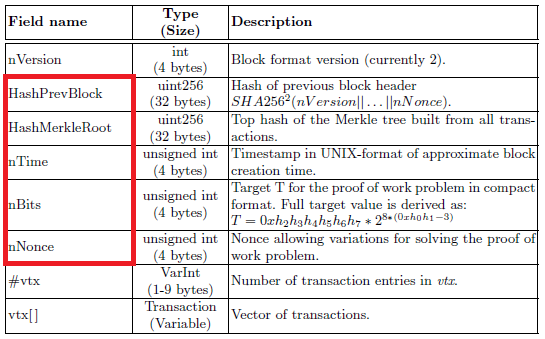
\includegraphics[scale=0.5]{bloque}
	\end{figure}
\end{frame}

\begin{frame}
\begin{block}{HashPrevBlock}
	Almacena la referencia al bloque anterior, calculada como un hash sobre el encabezado, tal como se describe en la siguiente imagen.
	\begin{figure}[h!]
		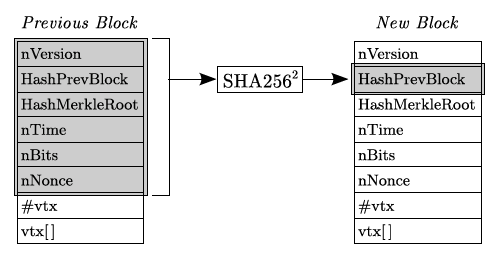
\includegraphics[scale=0.5]{referencia}
	\end{figure}
\end{block}
\end{frame}



\begin{frame}
	\begin{block}{HashMerkleRoot}
		Contiene la raíz del árbol de Merkle calculado a partir de las transacciones como datos y el doble $SHA256$ como función hash. 
	\end{block}\pause
\begin{block}{nTime}
	Almacena la marca de tiempo del momento aproximado de formación del bloque en formato UNIX. Se fija al inicio del proceso de formación del bloque.
\end{block}\pause
\begin{block}{nNonce}
	Contiene datos arbitrarios que se usan como fuente de aleatoriedad para resolver la prueba de trabajo.
\end{block}
\end{frame}

\begin{frame}
	\begin{block}{nBits}
		Contiene una representación compacta del valor objetivo $T$ de la prueba de trabajo. El valor $T$ tiene una longitud de 256 bits mientras que su forma compacta solo tiene 32 bits, con lo que se condifica con 8 dígitos hexadecimales. El valor objetivo se deriva de su forma compacta $0xh_0 h_1 h_2 h_3 h_4 h_5 h_6 h_7$ mediante la fórmula
		$$0xh_2h_3h_4h_5h_6h_7 \cdot 2^{8\cdot(0xh_0h_1-3)}$$
	\end{block}
\end{frame}

\begin{frame}
	Existe una cota superior para este valor, que se usó para minar el primer bloque (\emph{bloque génesis}), pero no una inferior. 
	
	Para asegurar un ritmo constante de 1 bloque minado cada 10 minutos, $T$ se recalcula cada 2016 bloques mediante la siguiente fórmula, donde $t_{sum}$ es el tiempo que se necistó para minar los 2015 bloques anteriores
	$$ T' =	\frac{t_{sum}}{14\cdot 24\cdot 60\cdot 60s}T$$
\end{frame}
\begin{frame}
	\begin{alertblock}{}
		En un bloque no se puede incluir dos veces la misma transacción ni transacciones que usen un mismo input, y tampoco se puede incluir una transacción que ya haya sido gastada en un bloque anterior (hay un orden cronológico), lo cual impide el doble gasto.
	\end{alertblock}
\end{frame}


\subsection{Minería}
\begin{frame}
	\frametitle{Formación de la cadena de bloques}
	
	\begin{defi}
		La \textbf{blockchain} es un registro de todas las transacciones ocurridas en el sistema de Bitcoin y se comparte con todos los nodos (dispositivos conectados) en él. Su propósito es poder determinar si una transacción ha sido gastada o no.
	\end{defi}\pause

Este registro adopta forma de cadena gracias a las referencias de cada bloque al bloque anterior, estableciendo así un orden cronológico.
\end{frame}

\begin{frame}
	\frametitle{Minería}
	\begin{defi}
		El proceso de encontrar un bloque válido y colocarlo en la blockchain se denomina \textbf{minería} y los nodos que lo llevan a cabo se llaman \textbf{mineros}. Los nodos que pueden realizar esta tarea se denominan \textbf{nodos completos}, es decir, nodos que tienen descargada toda la blockchain (en oposición a los \emph{nodos ligeros}, que veremos más adelante).
	\end{defi}
\end{frame}

\begin{frame}
	La minería consiste en lo siguiente:
	\begin{itemize}
		\item<2-> Recolectar las transacciones que cumplan los requisitos especificados por el minero (comisión recibida). Suelen recolectarse varios cientos de transacciones.
		\item<3-> Verificar las transacciones que se van a incluir en el bloque (verificar firma del pagador y prueba de conocimiento del receptor) y comprobar que sus inputs no han sido gastados previamente.
		\item<4-> Seleccionar el bloque más reciente en la blockchain (como veremos luego, puede ser necesario elegir entre varios) e insertar el hash del encabezado de ese bloque bloque en un nuevo bloque.
		\item<5-> Realizar la prueba de trabajo y publicarla para que pueda ser verificada.  %la red puede rechazarlo
	\end{itemize}
\end{frame}


\begin{frame}
	\href{https://www.blockchain.com/btc/unconfirmed-transactions}{Transacciones sin confirmar en tiempo real}
	
	\href{https://www.blockchain.com/btc/blocks}{Bloques minados hoy}
	
\end{frame}

\begin{frame}
	\frametitle{Prueba de trabajo}
	La prueba de trabajo en Bitcoin consiste concretamente en los siguientes pasos:
	\begin{itemize}
		\item<2-> Elegir un nonce en el campo $nNonce$ y el valor del campo $coinbase$.
		\item<3-> Calcular el hash del encabezado del bloque como
		\begin{gather*}
		SHA256^2(nVersion||HashPrevBlock||HashMerkleRoot||\\ nTime||nBits||nNonce)
		\end{gather*}
		
		\item<4-> Revertir el orden de los bytes del hash $H$ calculado anteriormente y comprobar que $H\leq T$ (el valor almacenado de forma compacta en $nBits$).
		\item<5-> En caso afirmativo, enviar la solución a la red, en caso contrario volver al primer paso.
	\end{itemize}
\end{frame}

\begin{frame}
	\frametitle{Fork}
	Una vez que los nodos completos validan las transacciones del bloque enviado y la prueba de trabajo, el minero recibirían los Bitcoins de recompensa junto con las comisiones. Sin embargo, puede pasar lo siguiente:
	
	\begin{itemize}
		\item<2-> Dos mineros resuelven sus pruebas de trabajo correspondiente aproximadamente al mismo tiempo. Sus bloques se confirman y son enviados a la red.
		\item<3-> Cada nodo completo recibirá primero uno de los dos bloques, con lo que comenzarán a trabajar en añadir otro bloque al primero que hayan recibido. El otro bloque lo mantendrán en reserva por si el siguiente bloque confirmado va detrás de ese.
	\end{itemize}
\end{frame}

\begin{frame}
	\begin{itemize}
		\item<1->  En este proceso llamado \textbf{fork} se divide la cadena como a continuación
		\begin{figure}
			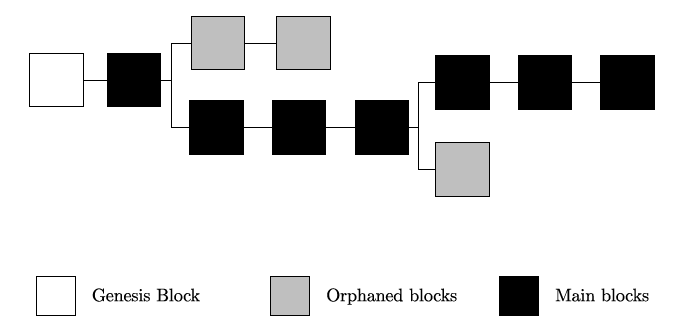
\includegraphics[scale=0.4]{fork}
		\end{figure}
	\item<2-> La rama que pervive es la que acumula más trabajo computacional (i.e. más mineros).
	\end{itemize}
\end{frame}

\begin{frame}
	Por este motivo se recomienda esperar hasta 6 bloques antes de aceptar una rama como rama principal. Después de esto, solo los mineros que tengan sus bloques en la rama principal reciben sus recompensas. Las transacciones de las otras ramas vuelven a quedar en espera para ser incluidas en otro bloque.
\end{frame}

\begin{frame}
	\href{https://anders.com/blockchain/}{Demo de Blockchain}
\end{frame}
\subsection{Nodos ligeros}
\begin{frame}
	\frametitle{Árboles de Merkle y nodos ligeros}
	El tamaño de la blockchain es de más de 200GB, por lo que no todos los nodos tienen capacidad para descargarla. Para poder comprobar que una transacción está en un bloque concreto se usan los árboles de Merkle.
	
	\begin{itemize}
		\item<2-> Supongamos que un bloque tiene $2^m$ transacciones indexadas por el conjunto de cadenas de $m$ bits de longitud y sea $n_i$, $i\in\{0,1\}^m$ el hash de la correspondiente transacción.
	\end{itemize}
\end{frame}

\begin{frame}
	\begin{itemize}
		\item<1-> Construimos el correspondiente árbol de Merkle
		\begin{figure}
			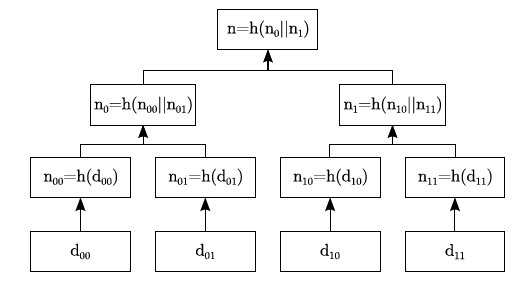
\includegraphics[scale=0.6]{merkle}
		\end{figure}
	\end{itemize}
\end{frame}

\begin{frame}
	\begin{itemize}
		\item<1-> Los \text{nodos ligeros} todo lo que tienen es el hash de la transacción $T$ y el encabezado del bloque que supuestamente lo contiene (en el cual está la raíz del árbol de Merkle del bloque).
		\item<2-> Para verificar que la transacción está efectivamente en ese bloque, con ayuda de un nodo completo se consiguen los $m$ hashes necesarios para reconstruir la rama correspondiente a $T$.
		\item<3-> Se reconstruye la rama y se comprueba que el último hash coincide con la raíz de árbol.
	\end{itemize}
\end{frame}

\begin{frame}
	\begin{itemize}
		\item Cada vez que dos transacciones que solo difieran en el último dígito de su índice sean gastadas, pueden ser borradas del registro, ya que no serán necesarias para verificar hashes.
		\item Eventualmente se pueden llegar a borrar ramas enteras que ni siquiera los nodos completos necesitarán.
	\end{itemize}
\end{frame}

\section{¿En qué consiste tener Bitcoin?}
\begin{frame}
	\frametitle{¿En qué consiste tener Bitcoin?}
	\begin{itemize}
		\item<1-> Para tener Bitcoin hace falta un \textbf{monedero}, esto es, una aplicación que genera una calve pública y una clave privada. El monedero tiene además una \textbf{dirección}. 
		\item<2-> Hay distintos tipos de dirección, pero básicamente son identificadores alfanuméricos de entre 26 y 35 caracteres. Se calculan hasheando sucesivamente la clave pública con $SHA256$ y $RIPEMD-160$ (reservando 4 bytes como checksum) y añadiendo al principio una componente constante que puede ser $1$, $3$ o $bc1$ (para reconocerlas como direcciones de Bitcoin). 
	\end{itemize}
\end{frame}

\begin{frame}
	\begin{itemize}
		\item<1-> El usuario no ve su clave pública sino su dirección. Así mismo, usa las direcciones de otros usuarios para enviarles Bitcoin.
		\item<2-> Una vez se tiene un monedero, la cantidad de Bitcoin del usuario no es más que la suma de los outputs de transacciones no gastadas que apuntan hacia la dirección del usuario.
	\end{itemize}
\end{frame}

\begin{frame}
	\begin{figure}
	
\includegraphics[scale=0.7]{bitcoin}
\end{figure}
\end{frame}

\end{document}
